\section{Pre-Processing}
Assume that we have a time-series system identification problem and we have \textbf{raw data}:
$$ \{y(1), y(2),...,y(N)\}$$
Before applying system identification techniques it is useful to check some \textbf{basic properties}:
\begin{itemize}
\item $E[y(t)]= m_y$ is \textbf{invariant} in time ( not time-dependent).
\item $\gamma_y(\tau) \xrightarrow[]{\tau \to \infty} 0 \to$ the process is \textbf{ergodic} so we can use \textbf{time-average} to compute \textbf{probabilistic} properties.
\item No data points are \textbf{missing}  
\end{itemize}
These properties are usually obtained by applying the following \textbf{pre-processing} techniques:
\begin{itemize}
\item \textbf{De-trend}
\item \textbf{Seasonal behaviour removal}
\item \textbf{Replacement of missing data}
\end{itemize}

\subsection{Removing a linear trend}
\begin{figure}[H]
 \centering
  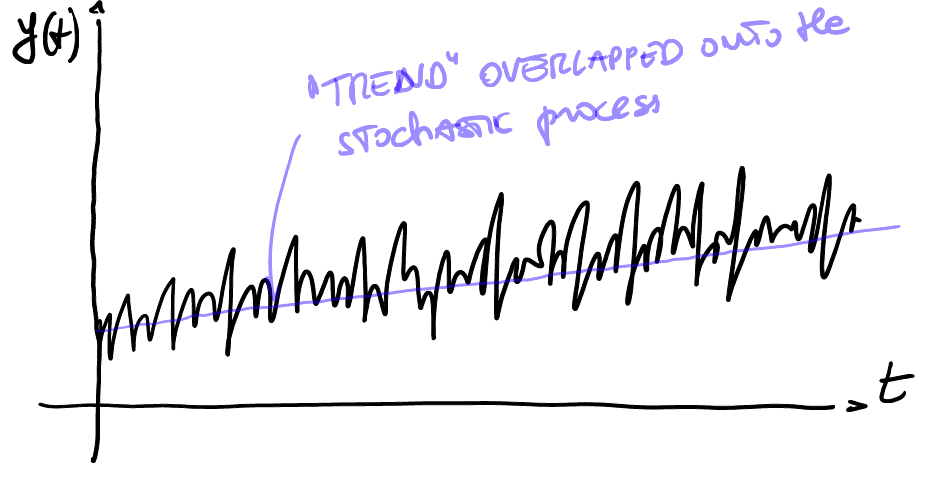
\includegraphics[width=.6\linewidth]{linear_trend}
\end{figure}
Model assumption : 
$$ y(t) = \tilde{y}(t) + kt+m$$
where
$$kt+m \text{ is a deterministic function of time (\textbf{trend})}$$
$$\tilde{y}(t) = \frac{C(Z)}{A(Z)}e(t) \text{ , zero-mean SSP}$$
\par\noindent\rule{\textwidth}{0.4pt}
\begin{description}
\item [Remark]\hfill\\
\begin{itemize}
\item k=0 $\to$ trend is simply a \textbf{bias} (trend of order 0)
\item Higher order trends like $k_3t^3+k_2t^2+k_1t+m$ (cubic trend)
\begin{figure}[H]
 \centering
  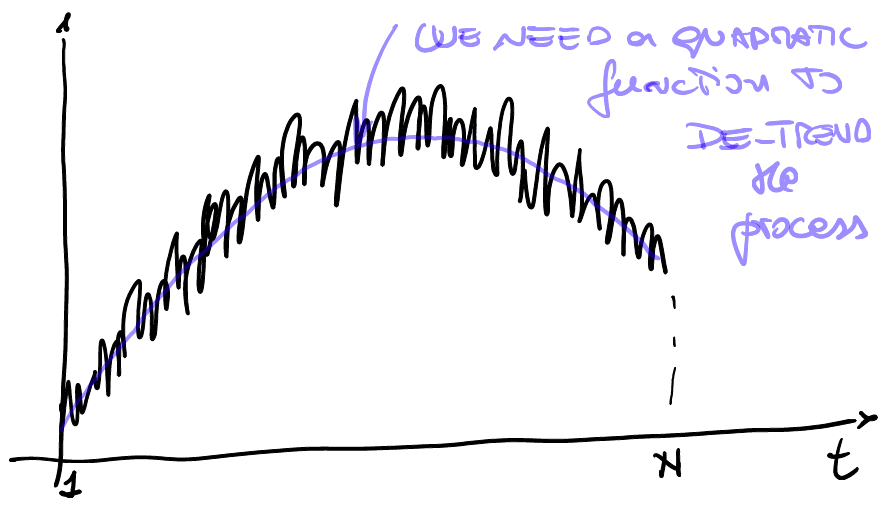
\includegraphics[width=.6\linewidth]{non_linear_trend}
\end{figure}
\end{itemize}
\end{description}
\par\noindent\rule{\textwidth}{0.4pt}
Assuming that the \textbf{linear trend} assumption is enough:
$$ y(t) = \tilde{y}(t) + kt+m$$
$$ E[y(t)] = E[\tilde{y}(t)] + E[kt+m]$$
$$ \begin{cases} 
	k \cdot 1 + m =y(1) \\ 
	k \cdot 2 + m =y(2) \\ 
	... \\
	k \cdot N + m =y(3)
	\end{cases}
$$
A system with N equations and 2 variables (\textbf{over-determined)}.\\
By solving the problem using a \textbf{least squares } approach :
$$\phi = \begin{bmatrix} 1 & 1 \\ 2 & 1 \\ .. & ..\\ N & 1 \end{bmatrix} , \theta=\begin{bmatrix} k \\ m \end{bmatrix}, Y = \begin{bmatrix} y(1) \\ y(2) \\ ... \\ y(N) \end{bmatrix}$$
$$ \phi \theta = Y \to \phi^T\phi\theta = \phi^TY$$
\[
\boxed{\hat{\theta} = \begin{bmatrix} \hat{k} \\ \hat{m} \end{bmatrix} = (\phi\phi^T)^{-1}\phi Y}
\]
So:
$$ \phi^T\phi =
 \begin{bmatrix} 1 & 2 & ... & N \\ 1 & 1 & ... & 1 \end{bmatrix} \cdot
  \begin{bmatrix} 1 & 1 \\ 2 & 1 \\ ... & ...\\ N & 1 \end{bmatrix} = 	   	 
  \begin{bmatrix} \sum\limits_{t=1}^{N}t^2 &  \sum\limits_{t=1}^{N}t \\ \sum\limits_{t=1}^{N}t & N \end{bmatrix}$$

$$ \phi^TY =
 \begin{bmatrix} 1 & 2 & ... & N \\ 1 & 1 & ... & 1 \end{bmatrix} \cdot
  \begin{bmatrix} y(1) \\ y(2) \\ ... \\ y(N) \end{bmatrix} = 	   	 
  \begin{bmatrix} \sum\limits_{t=1}^{N}t \cdot y(t)\\ \sum\limits_{t=1}^{N}y(t) \end{bmatrix}$$
  
\[
\boxed{\hat{\theta} = \begin{bmatrix} \hat{k} \\ \hat{m} \end{bmatrix} =\begin{bmatrix} \sum\limits_{t=1}^{N}t^2 &  \sum\limits_{t=1}^{N}t \\ \sum\limits_{t=1}^{N}t & N \end{bmatrix}^{-1} \begin{bmatrix} \sum\limits_{t=1}^{N}t \cdot y(t)\\ \sum\limits_{t=1}^{N}y(t) \end{bmatrix}}
\]
The same result can be found using:
$$\begin{bmatrix} \hat{k} \\ \hat{m} \end{bmatrix} argmin_{(k,m)}=\left\{ \frac{1}{N} \sum\limits_{t=1}^{N}(y(t) - kt-m)^2 \right\}  $$
Once $\hat{k} ,\hat{m}$ are found we can \textbf{de-trend} the data:
\[
\boxed{\tilde{y(t)} = y(t) - \hat{k}t-\hat{m}}
\]
If we wish to predict y(t):
$$\hat{y}(t+1|t)=\hat{\tilde{y(t)}}(t+1|t) + \hat{k}(t+1)+\hat{m}$$

\subsection{Removing seasonal behaviour}
In many practical applications some \textbf{seasonal} behaviour is overlapped to the main system dynamics. We assume a model of the \textbf{raw} dataset as follows:
$$ y(t) = \tilde{y}(t) + s(t) ,\text{ t=1,2,...N}$$
$$ \tilde{y}(t) = \frac{C(Z)}{A(Z)}e(t)$$
$$ s(t) \text{ is a periodic signal with period T : } s(t+kT)=s(t)$$
\par\noindent\rule{\textwidth}{0.4pt}
\begin{description}
\item [Remark]\hfill\\
\begin{itemize}
\item T is usually \textbf{a-priori known} ( a day, a week ,a year...)
\item It is possible to have multiple seasonal behaviour overlapped, where each component can be dealt with \textbf{independently}.
\item If T is \textbf{not} known a-priori, it is easy to \textbf{detect} it by a simple \textbf{FFT} of the raw signal
\begin{figure}[H]
 \centering
  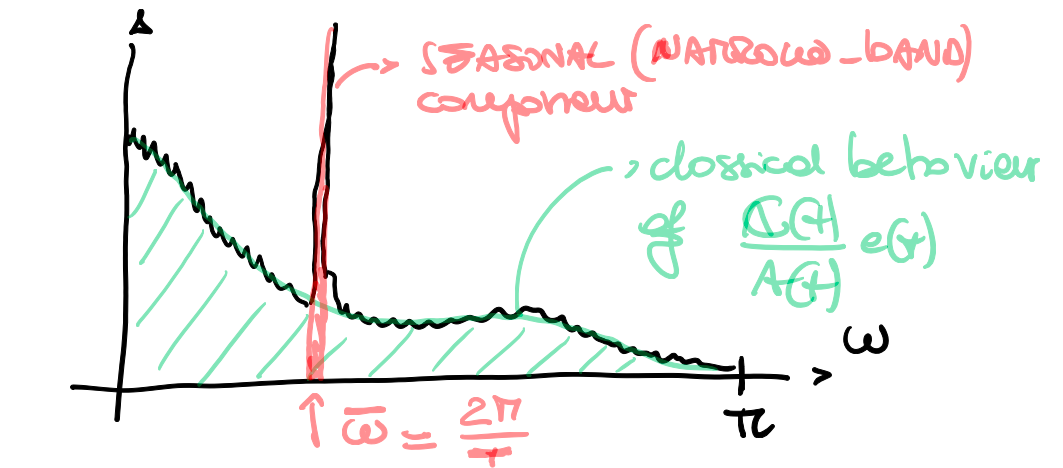
\includegraphics[width=.7\linewidth]{seasonal_fft}
\end{figure}
\item s(t) is \textbf{not a trend} $\to$  the process (raw data) y(t) can have \textbf{both} a trend and a seasonal behaviour. \textbf{FIRST} remove the trend \textbf{THEN} the seasonal behaviour.
\item If we don't remove a seasonal behaviour we end up with an \textbf{ARMA} model having a pair of \textbf{complex conjugate poles} at:
$$ e^{\pm j\Omega} , \Omega =\frac{2\pi}{T}$$  
\end{itemize}
\end{description}
\par\noindent\rule{\textwidth}{0.4pt}
The seasonal component of raw data can be estimated :
$$ t=1,2,3...N \text{  ,  } M\cdot T \leq N$$
\[
\boxed{\frac{1}{M}\sum\limits_{h=0}^{M-1}y(t+ht) \text{  , t=1,2,3...T}}
\]
\begin{figure}[H]
 \centering
  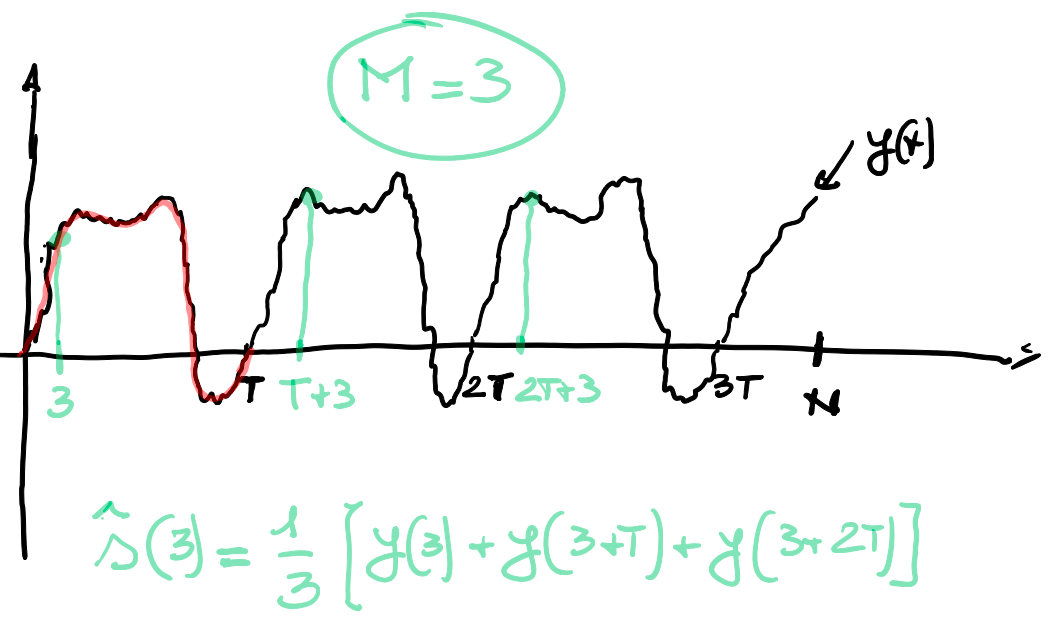
\includegraphics[width=.6\linewidth]{seasonal_est}
\end{figure}
\begin{figure}[H]
 \centering
  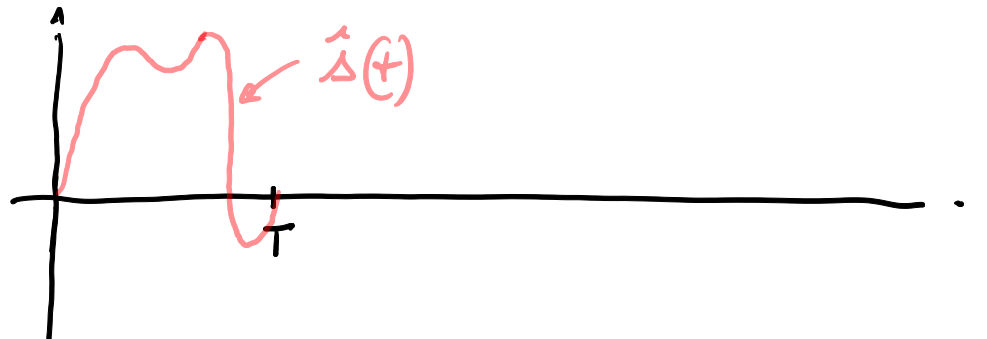
\includegraphics[width=.7\linewidth]{seasonal_est2}
\end{figure}
Once $\hat{s}$ is computed we can remove it from y(t).\\
After modelling $\tilde{y}(t)$ with an ARMA model the prediction will be:
\[
\boxed{\hat{y}(t+1|t) = \hat{\tilde{y}}(t+1|t) + \hat{s}(|t+1|_T)}
\]

\subsection{Missing data}
\begin{figure}[H]
 \centering
  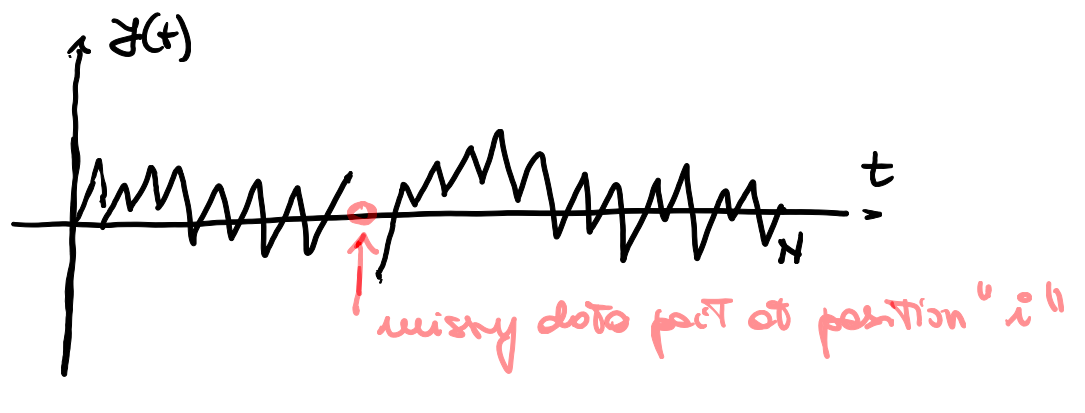
\includegraphics[width=.7\linewidth]{missing}
\end{figure}
Missing values are missing data points or \textbf{outliers} that are removed.
We need to fill in the data point $y(i)$ with an \textbf{estimated} one $\tilde{y}(i)$.
\subsubsection{Linear interpolation}
\[
\boxed{\tilde{y}(i) = \frac{y(i-1)+y(i+1}{2}}
\]
+: simple\\
-: does not work if we have \textbf{batch} of missing data points.

\subsubsection{Model estimation}
\begin{enumerate}
\item compute $\tilde{y}^{(1)}(i)$ using the linear interpolation method
\item using the complete dataset ( \textbf{including} $\tilde{y}^{(1)}(i)$ estimate a model for this dataset $\to m(\hat{\theta}^{(1)}_N)$
\item using the found model estimate $\tilde{y}(i)$ as 
\[
\boxed{\tilde{y}(i) = \hat{y}(i|i-1;\hat{\theta}^{(1)}_N)}
\] 
+:works also with a \textbf{batch} of missing data\\
-:more complex
\end{enumerate}
\newpage
\begin{description}
\item [Remark/Example]\hfill\\
I/O systems are the most typical situations where system identification techniques are used:
\begin{figure}[H]
 \centering
  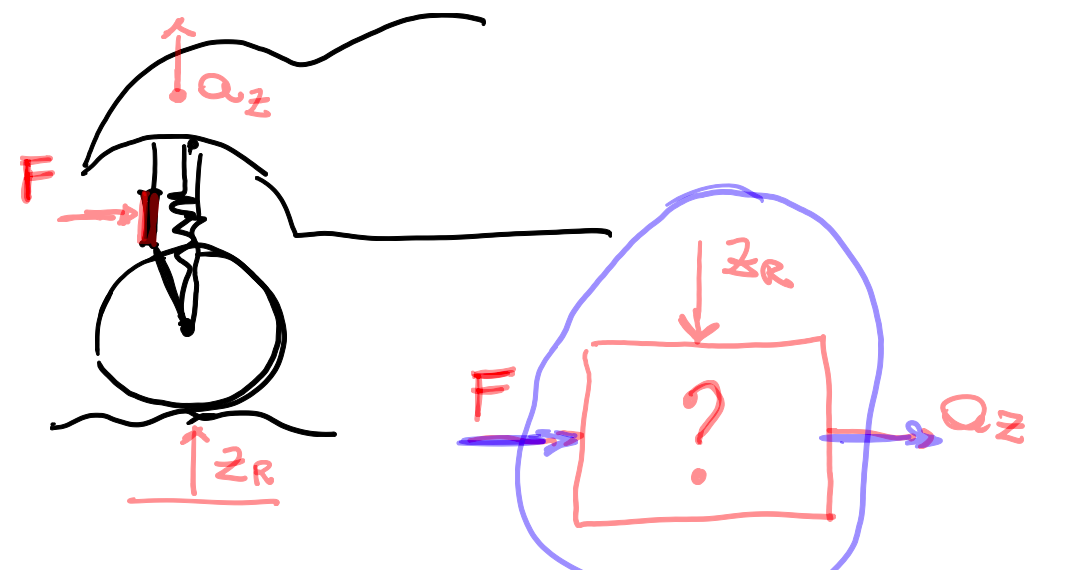
\includegraphics[width=.7\linewidth]{missing_example}
\end{figure}
In this example \textbf{F}$={F(1),...,F(N)}$ is the input signal and \textbf{a}$={a_z(1),...,a_z(N)}$ the output signal. We can estimate an \textbf{ARMAX} model:
\begin{figure}[H]
 \centering
  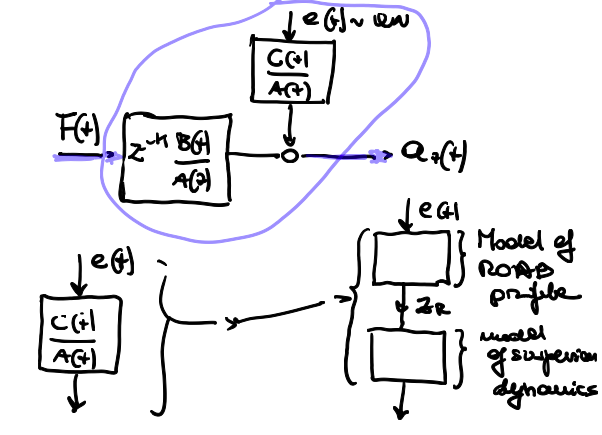
\includegraphics[width=.7\linewidth]{missing_example2}
\end{figure}
Neglecting the term e(t) (model of road profile and dynamics of suspension in this case) by taking in account only the input signal we end up with the \textbf{wrong} model which leads to the \textbf{wrong} description of the dynamics.
\end{description}
